\documentclass[12pt,twocolumn]{IEEEtran11}

\usepackage{times}
\usepackage{epsfig}
\usepackage[T1]{fontenc}
\usepackage{graphicx}
\usepackage{subfigure}
\def\BibTeX{{\rm B\kern-.05em{\sc i\kern-.025em b}\kern-.08em
    T\kern-.1667em\lower.7ex\hbox{E}\kern-.125emX}}

\oddsidemargin -15pt
\evensidemargin -15pt
\leftmargin 0 pt
\topmargin -30pt
\textwidth = 6.9 in
\textheight = 9.0 in

\newcommand{\itembase}{\setlength{\itemsep}{0pt}}
\newcommand{\eg}{{\it e.g., }}
\newcommand{\ie}{{\it i.e., }}
\graphicspath{{FIG/}}

\begin{document}
\bibliographystyle{IEEE}

\title{\Large \bf 
Survey on Bottlenecks and Best Practices of Three Implementations of
Distributed File Systems
}
\author{
Samuel Li\\
Information and Computer Science Department\\
University of Oregon\\
{\em samuelli@cs.uoregon.edu}
}
\maketitle
% You have to do this to suppress page numbers.  Don't ask.
%\pagestyle{empty}
\begin{abstract}
Filesystems are crutial components of supercomputers.
%
Often, filesystem of a supercomputer consists of many file servers
to provide capacity, performance, and reliability
required by a supercomputer.
%
These file servers are organized as a distributed system
to provide functionalities of a filesystem.
%
A distributed filesystem can have several performance challenges,
due to the distributed nature of the filesystem itself,
and the high concurrency nature of the supercomputer applications.
%
This survey paper studies performance issues of three widely 
used filesystems: Google File System,GPFS, and Lustre.
%
The scope of performance issues include identificatin of bottlenecks
and best approaches to minimize impact of these bottlenecks.
\end{abstract}

%\begin{keywords} 
%Quality Adaptive Streaming, Peer-to-Peer, Internet
%\end{keywords}

\section{Introduction}
\label{sec:intro}
File systems are a crucial component of many large-scale systems, 
namely the supercomputers and internet-based service providers.
%
While the computational capacity of modern supercomputers are keep growing,
the file system performance is not keep up the pace, in terms of both
the storage capacity and data transfer throughput.
%
Distributed file systems are widely used to tackle this problem.
%
On the one hand, distributed file systems enables a large number of commodity
storage devices to connect together and act like a unified storage space, 
which expands the storage capacity.
%
On the other hand, distributed file systems can potentially aggregate file
I/O operations from single storage devices together, providing a high
data transfer throughput. 
%
This survey paper sheds some light on the architecture as well as various
performance issues of distributed file systems.

%This survey paper identifies common performance issues in 
%the distributed file systems, 
%and explores approaches to minimize impacts of these issues.
%
This survey paper specifically looks into three popular distributed 
file systems: Google File System GPFS, and Lustre.
%
Google File System~\cite{ghemawat2003google} is designed by Google and used 
exclusively by Google.
%
GPFS~\cite{Schmuck2002,barkes1998gpfs} is a proprietary system owned by IBM, and
it also powers many supercomputers.
%
Lustre~\cite{Schwan2003} is open-sourced and powers many of the 
world's fastest supercomputers.
%
We will especially focused on three aspects of these file systems:
1) different architecture design,
2) file partitioning scheme, and 3) efforts and demonstrations to achieve
higher performance using these three file systems.


\section{Architecture of Three Filesystems}
\label{sec:architecture}
\subsection{Google File System}
\label{sec:archi_google}
%
\begin{figure*}
\centering
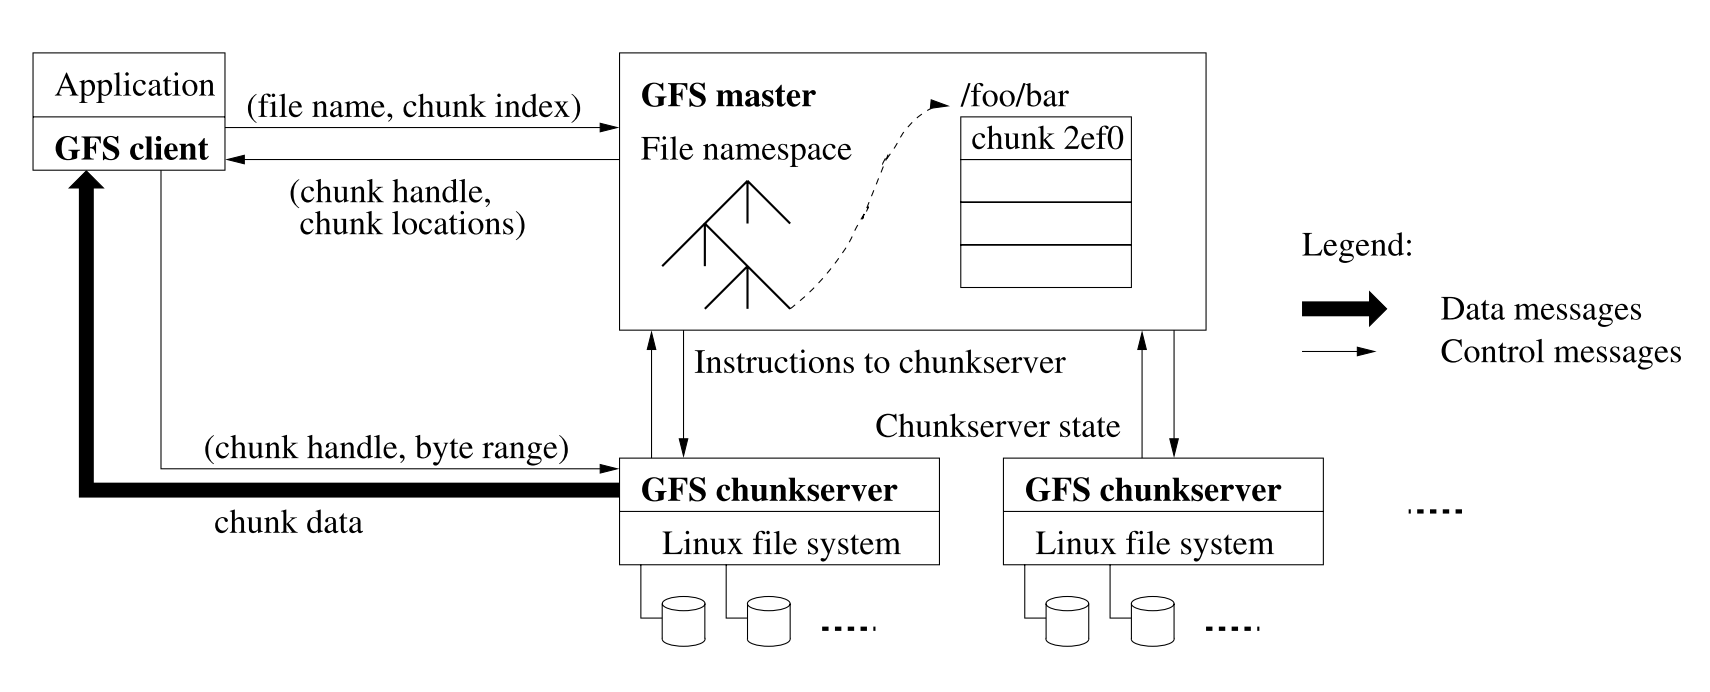
\includegraphics[width=0.95\textwidth]{image/gfs_architecture.png}
\caption{GFS architecture}
\label{fig:gfs_architecture}
\end{figure*}
%
The Google filesystem is the proprietary file system designed by 
Google~\cite{ghemawat2003google}.
%
It has a few impressive properties, such as the ability to reach a global
scalability~\cite{Ford2010a,Corbett2012a}, and the good performance on 
structured data~\cite{Chang2006a}.
%
However, publications are limited due to its proprietary nature. 
%
This section gives an overview of Google filesystem (GFS) based on the available
publications.

The initial design choices of GFS are explained by 
Ghemawat et al.~\cite{ghemawat2003google}.
%
It started from four observations regarding the unique usages and 
requirements by Google:
%
\begin{enumerate}
\item ``component failures are the norm rather than the exception";
\item ``files are huge by traditional standards";
\item ``most files are mutated by appending new data
		rather than overwriting existing data"; and
\item ``co-designing the applications and the file system API benefits the 
		overall system by increasing our flexibility."
\end{enumerate}
%
The extra flexibility as described by the fourth item enables GFS to 
make some radical design choices, for example, it does not comply to
any standard API.
%
In contrast, the other two surveyed filesystems both comply the 
standard API of POSIX.
%
We will revisit these observations and discuss how they
impact the design of GFS in the following discussion.


\subsubsection{Master-Server Architecture: Master}
GFS adopts a master-server architecture.
%
More specifically, each GFS cluster consists of one master node and 
multiple chunkservers; both are commodity machines.

The roles of master include:
\begin{enumerate}
\item maintaining all filesystem metadata, including
	namespace, access control, mapping from files to chunks, and current
	locations of chunks;
\item monitoring system state by sending periodical heartbeat messages and 
	collecting system state of individual chunkservers;
\item controlling system-wide activities, such as lease management, 
	garbage collection, chunk migrations; and
\item answering requests from clients.
\end{enumerate}

Because there is only one single master node in a GFS system, the master can
easily become a system bottleneck.
%
To prevent this from happening, the master takes a minimum involvement
in the fourth task: answering requests from clients.
%
More specifically, the master does not handle any of the actual file I/O
operations; rather, it sends instructions and re-directs actual file I/O 
operations to the proper chunkserver nodes.
%
These instructions include which chunkservers to look for, and what chunk 
handles to use.
%
Clients then interact with file chunkservers to finish the actual file I/O 
operations.


\subsubsection{Master-Server Architecture: Chunkserver}
The chunkservers in GFS are machines that actually stores data files.
%
Data is stored as chunks in GFS, so each chunkserver stores many data chunks.
%
The chunk size is an important parameter to tune the GFS, and 
64MB is decided to be a good balance between disk utilization and 
system performance.
%
%A file server always listens instructions from the master to perform 
%routine tasks, including:
A chunkserver always performs tasks from either instructions from the 
master, or the clients. 
%
Typically, these tasks include:
%
\begin{enumerate}
\item read and write operations per requests by clients;
\item maintenance tasks such as replicating an existing data chunk;
\item lease management, including requiring a lease, extending a lease, 
	and releasing a lease; and
\item rallying in a data flow along a chain of chunkservers. 
\end{enumerate}
%
We will discuss the last task in Section~\ref{}.

The overview of GFS architecture is shown in Figure~\ref{fig:gfs_architecture}.



\subsection{IBM GPFS: General Parallel File System}
\label{sec:archi_gpfs}
%
\begin{figure}
\centering
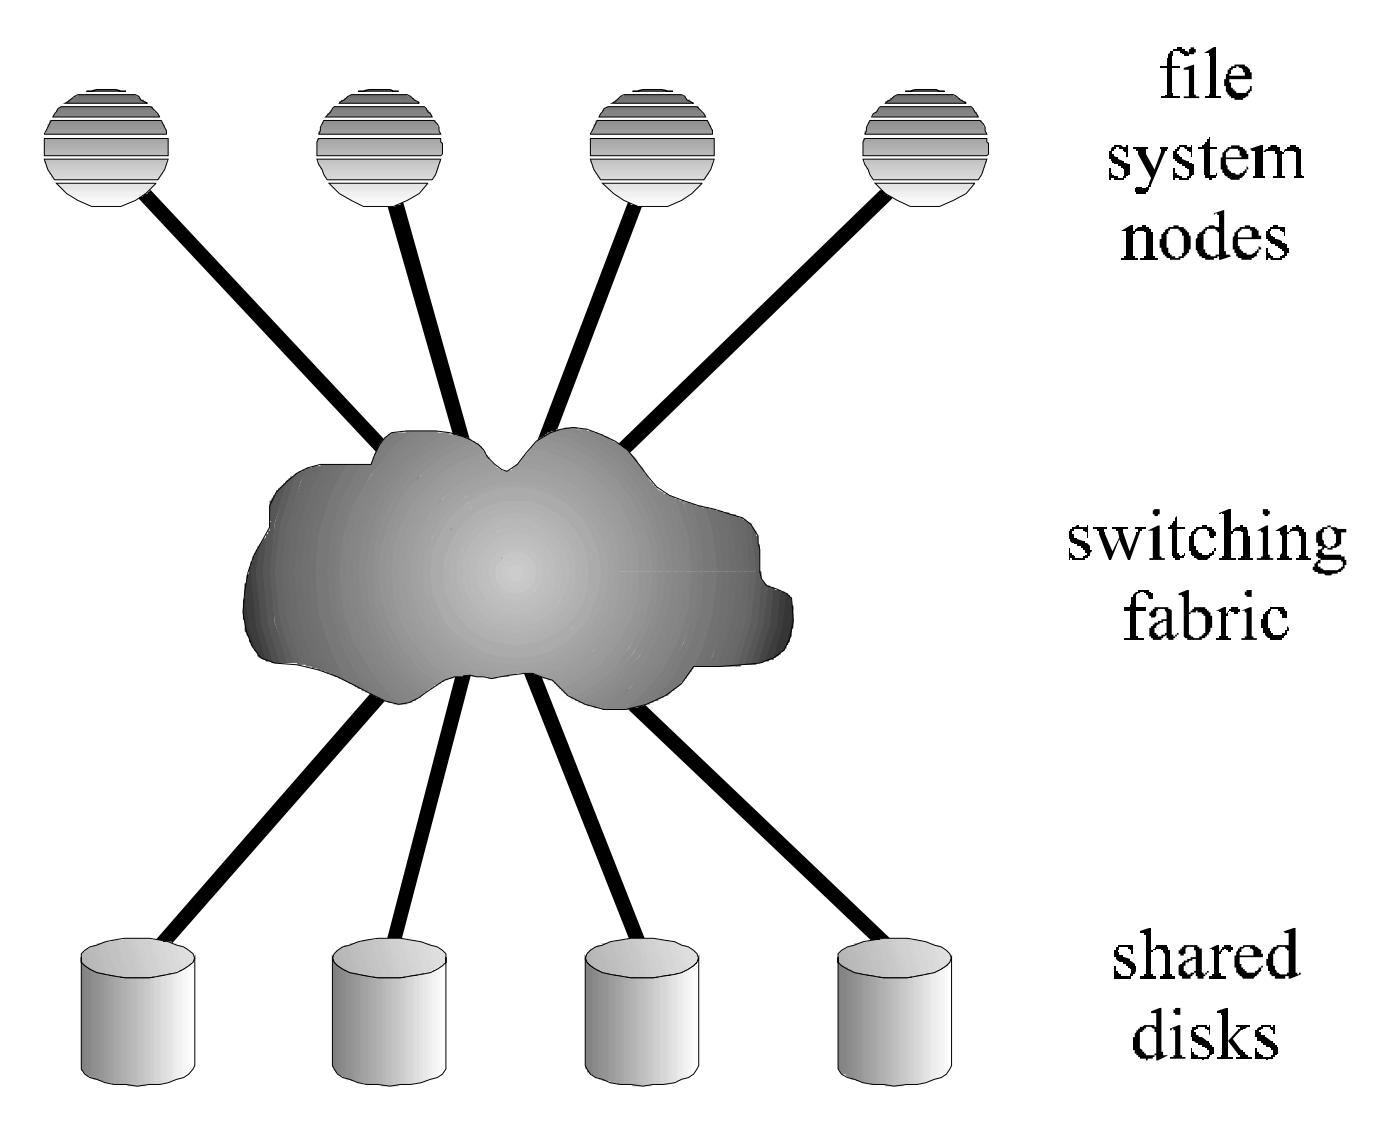
\includegraphics[width=0.95\columnwidth]{image/gpfs_architecture.png}
\caption{GPFS architecture}
\label{fig:gpfs_archi}
\end{figure}
%
The General Parallel File System (GPFS) from IBM is a popular filesystem
that is more widely adopted than the Google File System. 
%
In fact, it powers some of the most powerful supercomputers in the world,
including the third and fifth fastest supercomputers (Sequoia and Mira 
respectively) in the latest Top500 list~\cite{Strohmaier:2006:TS:1188455.1188474}.
%
Accordingly, there is more published research on GPFS than GFS.
%
However, because of the proprietary nature of GPFS, the publications on 
GPFS is also relatively limited. 
%
We provide an overview of the architecture of GPFS in this section.


\subsubsection{Decentralized Architecture}
GPFS adopts a decentralized architecture.
%
More specifically, there are cluster nodes and disks or disk subsystems.
%
Clusters and disks are connected over a switching fabric.
%
The architecture is decentralized in the sense that all cluster nodes 
have equal to the disks, and they provide equal functionalities and access
to user applications.

Data stored on GPFS is distributed into many stripes, and are essentially
placed on different disks.
%
This design enables parallel data access, which helps improving the overall
I/O performance.
%
We will discuss more about this parallel data access later in Section~\ref{}.

The locking mechanism of GPFS is mostly distributed as well with a few tasks
performed in a centralized fashion.
%
The centralized locking routines mainly takes care of updates on metadata
and configuration files.
%
Even these routines are centralized, the central coordinator is elected from
the pool of clusters, and can hardly run into a single-point failure problem.
%
Figure~\ref{fig:gpfs_archi} provides an overview of the GPFS architecture.



\subsection{Lustre File System}
\label{sec:archi_lustre}
%
\begin{figure}
\centering
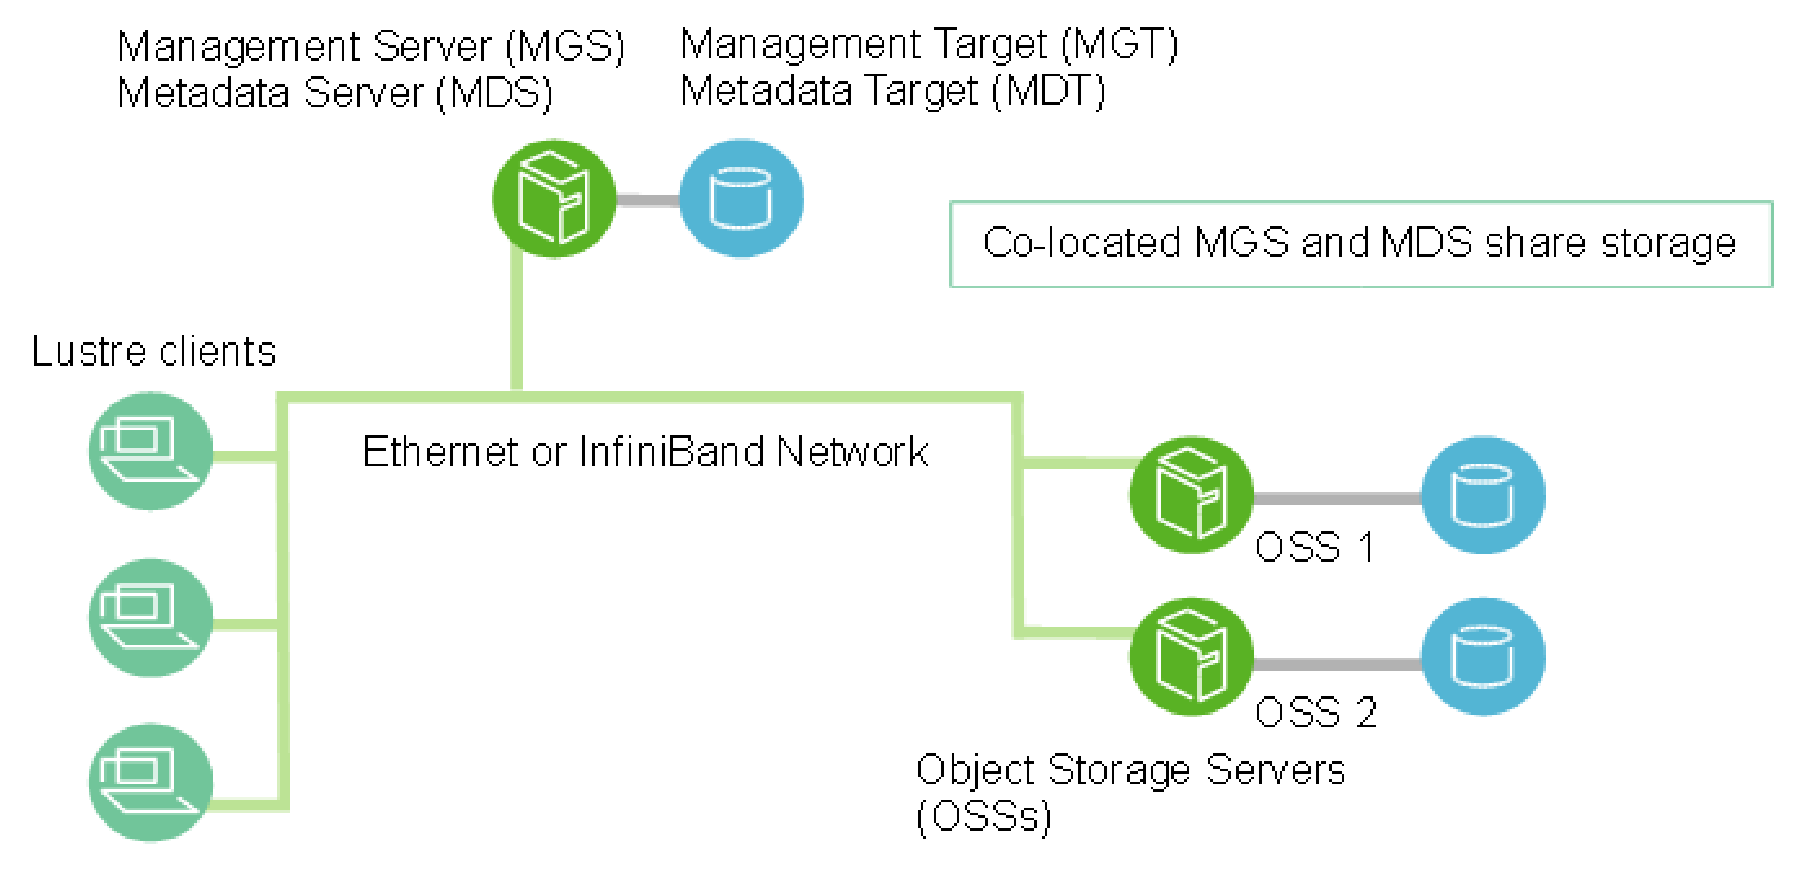
\includegraphics[width=0.99\columnwidth]{image/lustre_architecture.png}
\caption{Lustre architecture}
\label{fig:lustre_archi}
\end{figure}
%
Lustre is an open-sourced filesystem. 
%
Like GPFS, Lustre has also been used by many of the world's top supercomputers.
%
It is also the most intensively researched distributed file system among 
the three. 

\subsubsection{Lustre File System Architecture}
The Lustre file system has a similar architecture as GFS:
one node serves as management server (MGS); 
multiple object storage servers (OSS) actually stores data;
management server and object storage servers are connected via
high-speed network.
%
It should also be noted that later releases of Lustre do have support
for multiple metadata servers to provide better reliability.

On the management server side, it keeps all the metadata in object files,
named metadata target (MDT).
%
MDTs have information filenames, directories, permissions and file layout.
%
The MGS also provides network request handlings for local MDTs.

On the object storage server side, data is grouped as object storage targets
(OSTs). 
%
The mapping between OSSs and OSTs can be flexible, which means 
one OSS can have multiple OSTs, or
multiple OSSs have access to one OST, or
even a more complex $n$ to $m$ mapping.
%
The final choice of mapping scheme is based on the usage and the choice of 
hardware. 
%
For example, one OSS can host two OSTs to achieve redundency if using 
commodity storage, while utilize the complex $n$ to $m$ mapping to achieve
high performance if using enterprise-class storage arrays.
%
Figure~\ref{fig:lustre_archi} provides an overview of the Lustre architecture.


\subsection{Discussion on Three Architectures}
The three surveyed filesystems, GFS, GPFS, and Lustre represent two 
distinct architectures: architecture with a master node or 
architecture without a master node.
%
Both architectures have advantages and disadvantages.

GFS, Lustre have a master node, and this design has a major advantage
that it is easy to perform maintenance creating data replica; 
migrating partial data; detecting and 
from failures; communicating with clients; etc.
%
The master node has this advantage because it possesses a global knowledge
of the entire file system.
%
The disadvantage is also obvious that the master node can cause a 
single-point failure.
%
This disadvantage can be largely avoided by providing a replica of the master
node, as what Lustre does.
%
A less severe drawback is that the master node can become a system bottleneck.
%
Modern supercomputers tend to equip a large amount of memory and fast storage
such as solid state drives to tackle this problem.

GPFS uses a decentralized architecture without a master node.
%
This design has an obvious advantage that it has better tolerance on 
failure of single nodes.
%
This property is quite important on large scale systems.
%
The disadvantage of this decentralized architecture is that implementation
of many operations, like locks or leases, becomes complicated in many cases.
%






\section{Briefs}
\label{sec:brief}
%The following papers characterize behaviors of distributed file systems
%on supercomputers:
%\cite{Xie2012}, \cite{Henschel2012}, \cite{Crosby2009}, \cite{Borrill2009}.

%The following papers discuss approaches to better work with distributed 
%file systems given the characters above:
%\cite{Shipman2010}, \cite{Yu2006}, \cite{Tian2011}, \cite{Lofstead2010},
%\cite{Lofstead2009}.

\subsection{Research on Lustre}
Many research papers have focused on the performance issue of 
Lustre file systems. 
%
Here is a selected collection and the main topic of each paper:
Crosby~\cite{Crosby2009} characterized the performance of Lustre file system
on a real supercomputer system;
%
Xie et al.~\cite{Xie2012} specifically characterized output performance
with respect to a number of system parameters;
%
Schwan~\cite{Schwan2003} and Henschel et al.~\cite{Henschel2012} 
demonstrate implementations of Lustre to achieve the best performance
on real systems; 
%
Lofstead~\cite{lofstead2010managing} et al. specifically researched interference effects
measured on two real systems; and
%
Shipman et al.~\cite{Shipman2010} summarized real lessons learned 
to achieve high performance on a very large scale Lustre file system.


\subsection{Research on GPFS}
GPFS comes with most IBM supercomputers, and also receives intense study
in terms of its performance.
%
Yu et al.~\cite{Yu2006} demonstrated a highly scalable GPFS file system
with satisfactory overall performance;
%
Andrews et al.~\cite{Andrews2005} researched from both theoratical 
and practical sides of the performance of GPFS file system
in an inter-state scale.
%
Further, Freitas et al.~\cite{freitas2011gpfs} reported performance 
of GPFS file system to scan 10 billion files in 43 minutes. 


\subsection{Research on Google File System}
Even Google intends to keep the Google File System restrict
to its own use, it still publishes a few papers discussing the 
performance of Google File System.
%
In addition to the original paper that specifies the design of
Google File System~\cite{ghemawat2003google},
Chang et al.~\cite{Chang2006a} also discusses efforts to make Google
File System better handle structured data;
Ford et al.~\cite{Ford2010a} and Corbett et al.~\cite{Corbett2012a}
also disscussed how Google File System achieves a global scalability.


The rest of this survey paper will elaborate above mentioned studies 
to provide a big picture on performance issues of parallel file systems
and available approaches to best make use of these systems.


%% file citations.bib contains all the biblography
\bibliography{main}
\end{document}
